\documentclass[12pt]{article}
\usepackage{paralist}
\usepackage{tikz}
\usepackage{float}
\usepackage{graphicx}
\usepackage[font=small,labelfont=bf]{caption}
\usepackage{subcaption}
\usepackage{multirow}
\usepackage{balance}

\pagenumbering{gobble}

\title{Figures}
\author{}

%%%%%%%%%%%%%%%%%%%%%%%%%%%%%%%%%%%%%%%%%%%%%%%%%%%%%%%%%%%%%%%%%%%%%%%%%%%%%%%%
\begin{document} %%%%%%%%%%%%%%%%%%%%%%%%%%%%%%%%%%%%%%%%%%%%%%%%%%%%%%%%%%%%%%%

\begin{figure}
\centering
\begin{tabular}{|l|r|}
\hline
View Type               & Mean Encoding Time per Frame (secs.) \\
\hline
Independent             & 4.65                                 \\
Dependent, 1 reference  & 3.48                                 \\
Dependent, 2 references & 13.39                                \\
\hline
\end{tabular}
\caption{
Time to encode a frame of each view type averaged over 100 frames and 10 trials
with each data-set.
}
\end{figure}

\begin{figure}
\centering
\begin{subfigure}{.4\textwidth}
\centering
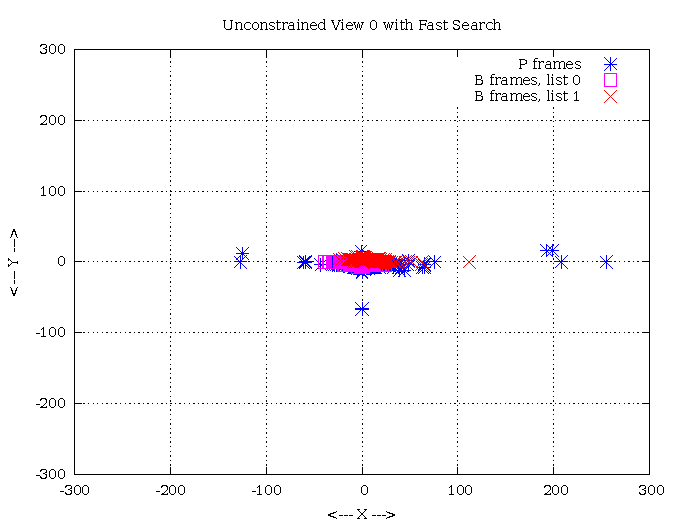
\includegraphics[width=2.75in]{figures/bedroom1-inter-mvs.eps}
\caption{Bedroom data set.}
\end{subfigure} \hspace{.8in}
\begin{subfigure}{.4\textwidth}
\centering
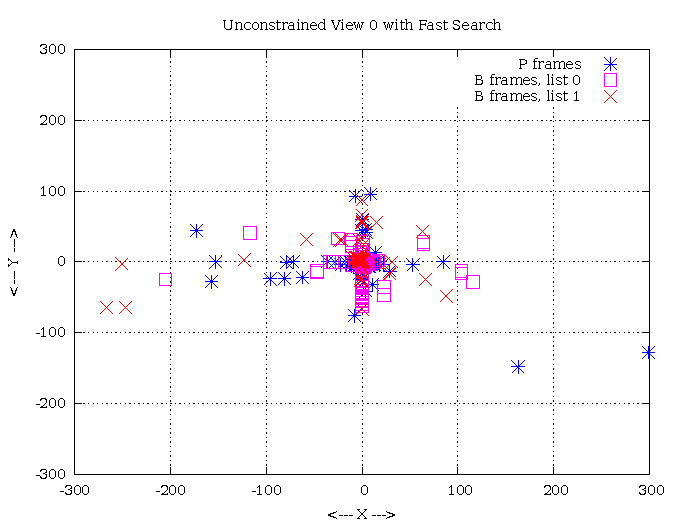
\includegraphics[width=2.75in]{figures/helicopter-inter-mvs.eps}
\caption{Helicopter data set.}
\end{subfigure}
\caption{Independent view (inter) motion vectors from the 2-view test of each data set.}
\end{figure}

\begin{figure}
\centering
\begin{subfigure}{\textwidth}
\centering
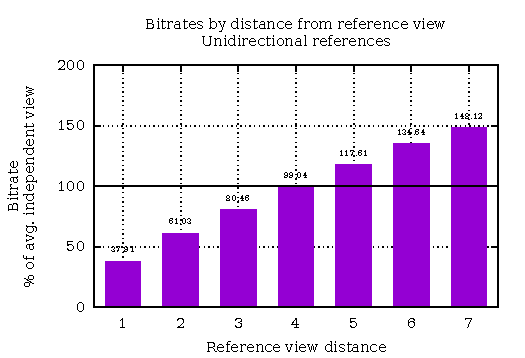
\includegraphics[scale=1]{figures/motion_vector_data_unconstrained_unidirectional.eps}
\caption{Dependent views with one reference.}
\end{subfigure} \\ \vspace{.3in}
\begin{subfigure}{\textwidth}
\centering
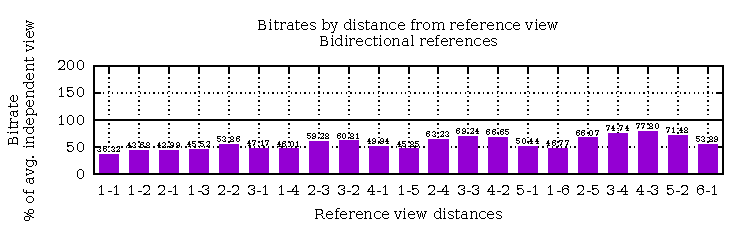
\includegraphics[scale=1]{figures/motion_vector_data_unconstrained_bidirectional.eps}
\caption{Dependent views with two references.}
\end{subfigure}
\caption{Average bit-rate by distance from the reference view.}
\end{figure}

%\begin{figure}
%\centering
%\begin{subfigure}{.4\textwidth}
%\centering
%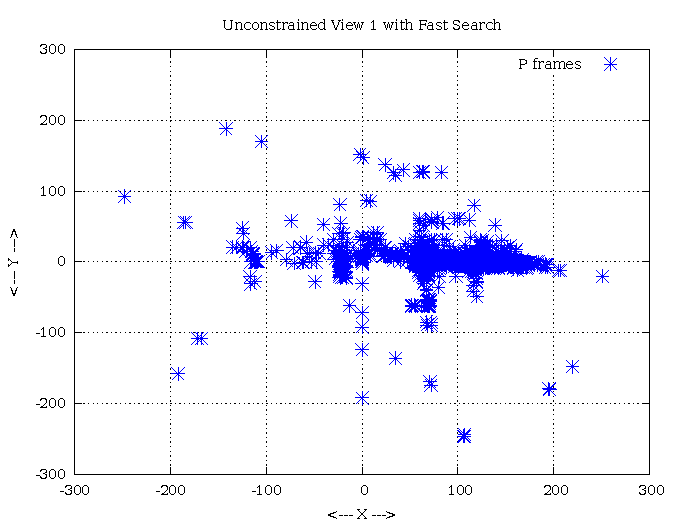
\includegraphics[width=2.75in]{figures/bedroom1-inter-view-mvs.eps}
%\caption{Bedroom data set.}
%\end{subfigure} \hspace{.8in}
%\begin{subfigure}{.4\textwidth}
%\centering
%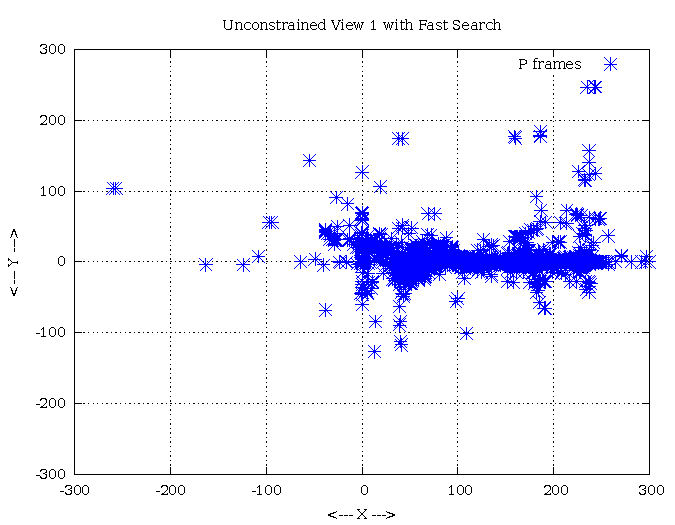
\includegraphics[width=2.75in]{figures/helicopter-inter-view-mvs.eps}
%\caption{Helicopter data set.}
%\end{subfigure}
%\caption{Unconstrained inter-view motion vectors from 2-view test of each data-set (one reference).}
%\end{figure}

%\begin{figure}
%\centering
%\begin{subfigure}{.4\textwidth}
%\centering
%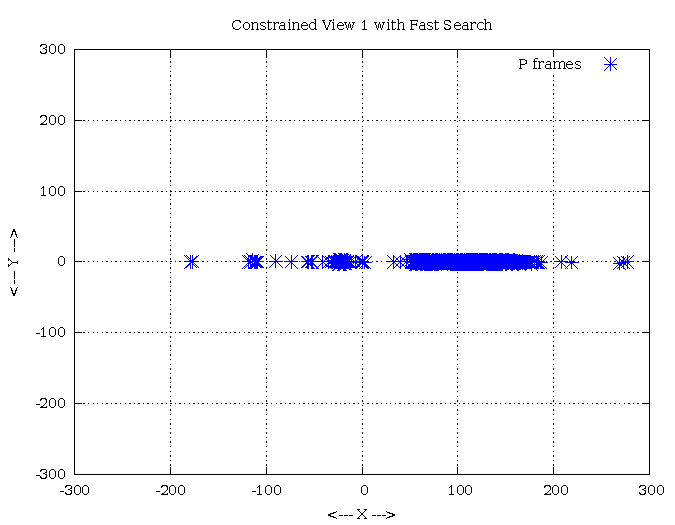
\includegraphics[width=2.75in]{figures/bedroom1-inter-view-constrained-mvs.eps}
%\caption{Bedroom data set.}
%\end{subfigure} \hspace{.8in}
%\begin{subfigure}{.4\textwidth}
%\centering
%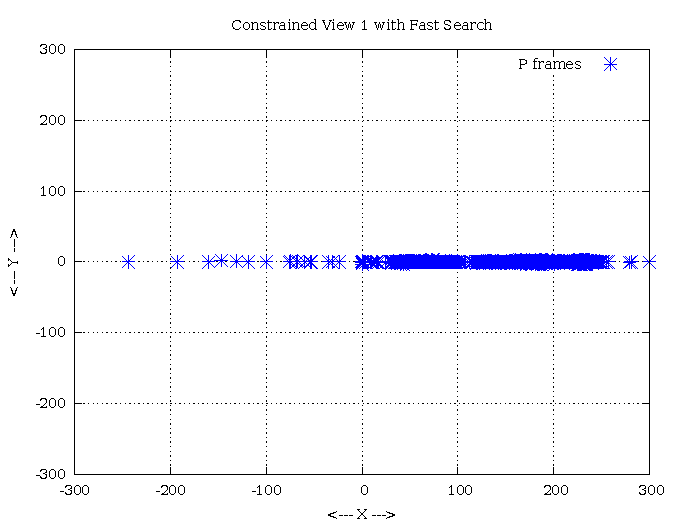
\includegraphics[width=2.75in]{figures/helicopter-inter-view-constrained-mvs.eps}
%\caption{Helicopter data set.}
%\end{subfigure}
%\caption{Constrained inter-view motion vectors from 2-view test of each data-set (one reference).}
%\end{figure}

\begin{figure}
\centering
\begin{subfigure}{.4\textwidth}
\centering
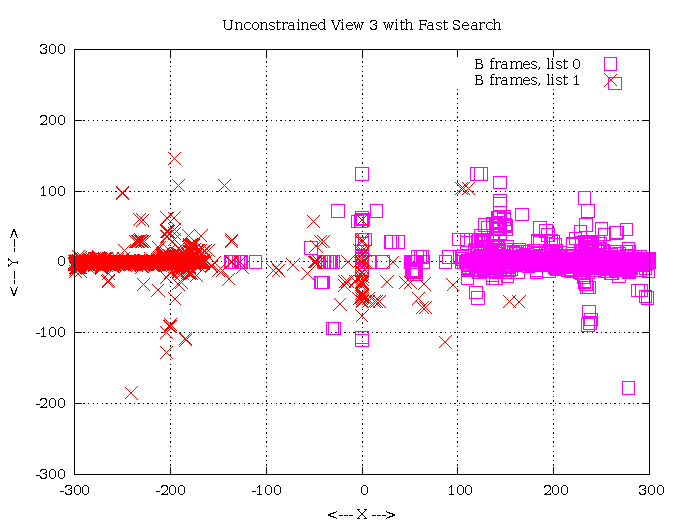
\includegraphics[width=2.75in]{figures/bedroom1-inter-view-bimvs1.eps}
\caption{View 3 of the bedroom data set.}
\end{subfigure} \hspace{.8in}
\begin{subfigure}{.4\textwidth}
\centering
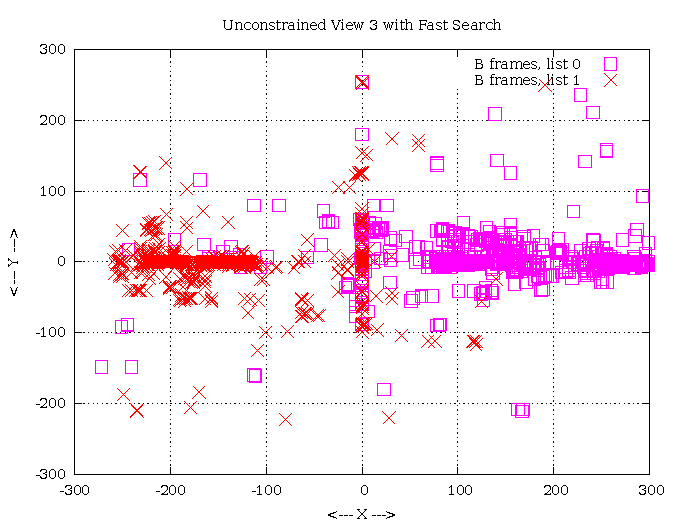
\includegraphics[width=2.75in]{figures/helicopter-inter-view-bimvs1.eps}
\caption{View 3 of the helicopter data set.}
\end{subfigure} \\ \vspace{.3in}
\begin{subfigure}{.4\textwidth}
\centering
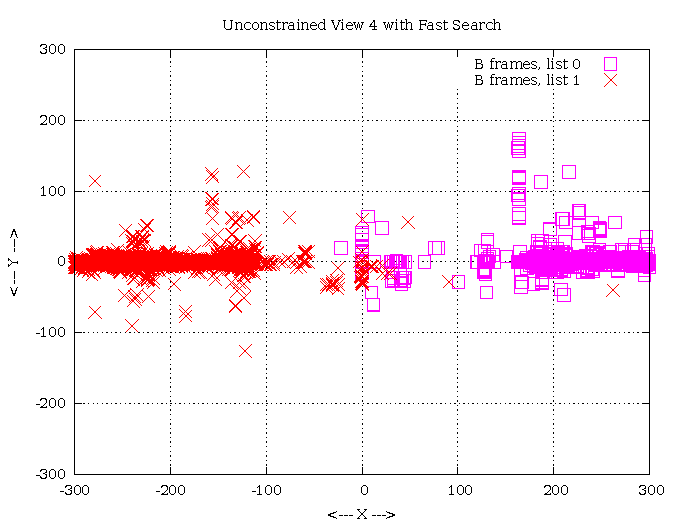
\includegraphics[width=2.75in]{figures/bedroom1-inter-view-bimvs2.eps}
\caption{View 4 of the bedroom data set.}
\end{subfigure} \hspace{.8in}
\begin{subfigure}{.4\textwidth}
\centering
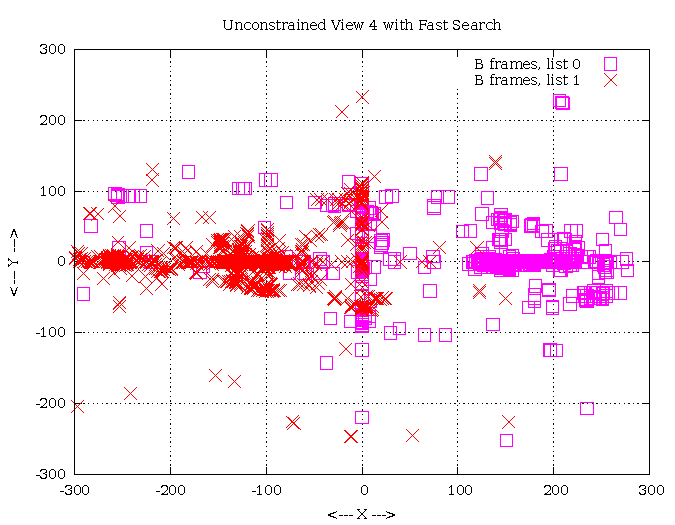
\includegraphics[width=2.75in]{figures/helicopter-inter-view-bimvs2.eps}
\caption{View 4 of the helicopter data set.}
\end{subfigure}
\caption{
Unconstrained inter-view bidirectional motion vectors from views 3 and 4  of the
8-view test of each data-set.
}
\end{figure}

\begin{figure}
\centering
\begin{subfigure}{.4\textwidth}
\centering
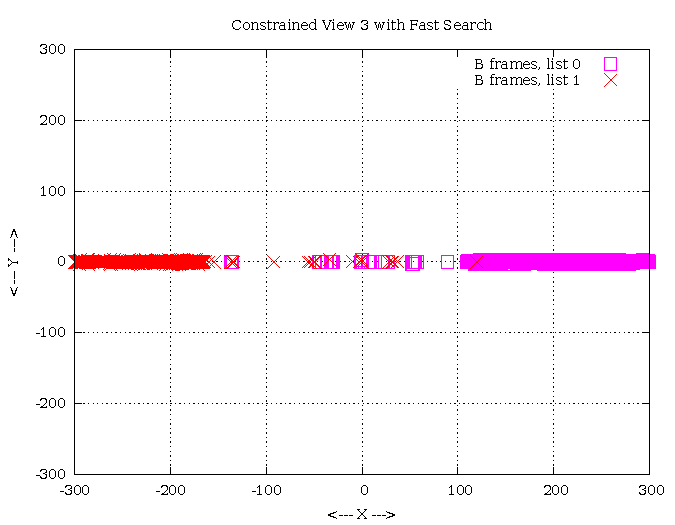
\includegraphics[width=2.75in]{figures/bedroom1-inter-view-constrained-bimvs1.eps}
\caption{View 3 of the bedroom data set.}
\end{subfigure} \hspace{.8in}
\begin{subfigure}{.4\textwidth}
\centering
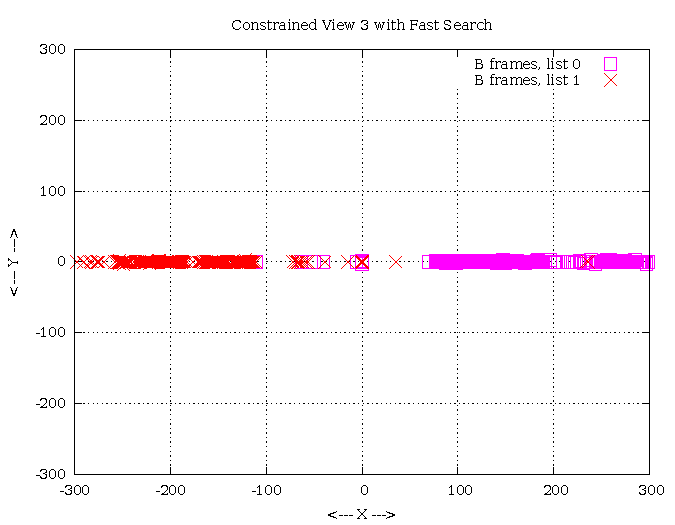
\includegraphics[width=2.75in]{figures/helicopter-inter-view-constrained-bimvs1.eps}
\caption{View 3 of the helicopter data set.}
\end{subfigure} \\ \vspace{.3in}
\begin{subfigure}{.4\textwidth}
\centering
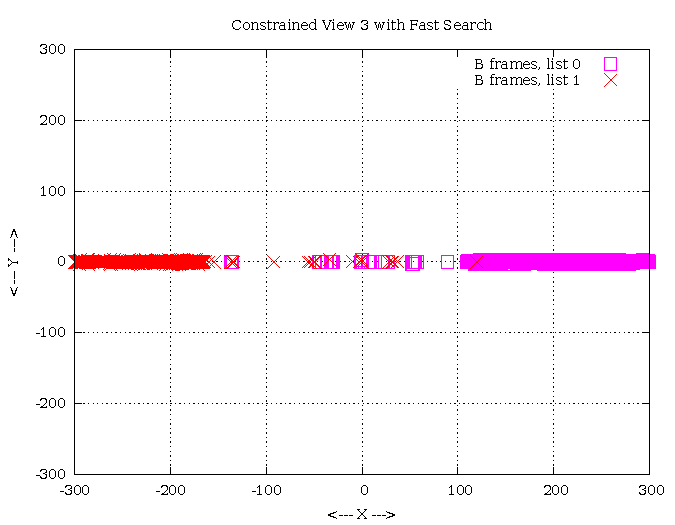
\includegraphics[width=2.75in]{figures/bedroom1-inter-view-constrained-bimvs1.eps}
\caption{View 4 of the bedroom data set.}
\end{subfigure} \hspace{.8in}
\begin{subfigure}{.4\textwidth}
\centering
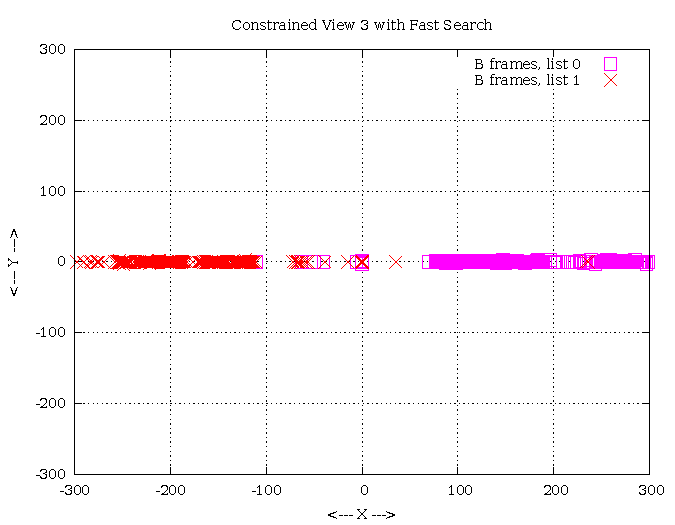
\includegraphics[width=2.75in]{figures/helicopter-inter-view-constrained-bimvs1.eps}
\caption{View 4 of the helicopter data set.}
\end{subfigure}
\caption{
Constrained bidirectional dependent view motion vectors from the views 3 and 4
of the 8-view test.
}
\end{figure}

\pagebreak
\begin{figure}
\centering\small
\begin{tabular}{|l|l|l|l|l|}
\multicolumn{1}{c}{} & \multicolumn{2}{c}{Unconstrained} & \multicolumn{2}{c}{Constrained} \\ \hline
Algorithm            & Bits            & Secs.           & Bits            & Secs.         \\ \hline
Full                 & 20935.92        & 142.58          & 22488.00        & 2.37          \\ \hline
TZ-search            & 21136.80        & 2.72            & 22551.12        & 1.43          \\ \hline
\end{tabular}
\caption{
Seconds and bits per encoded frame of the dependent view of the 2-view test
using full and TZ-search (100 frames).
}
\end{figure}

\begin{figure}
\centering\small
\begin{subfigure}{.5\textwidth} \hspace{-.6in}
\begin{tabular}{|l|l|l|l|l|l|}
\multicolumn{2}{c}{} & \multicolumn{2}{c}{Unconstrained} & \multicolumn{2}{c}{Constrained} \\ \hline
View & Num. Refs.    & Bits            & Secs.           & Bits            & Secs.         \\ \hline
0    & 1             & 17503.73        & 2.74            & 17806.24        & 1.45          \\ \hline
2    & 1             & 18294.58        & 2.67            & 18751.60        & 1.44          \\ \hline
3    & 2             & 30397.04        & 11.88           & 30416.96        & 3.03          \\ \hline
4    & 2             & 30430.88        & 11.47           & 30398.82        & 2.93          \\ \hline
5    & 1             & 18661.41        & 2.62            & 19044.34        & 1.51          \\ \hline
7    & 1             & 19802.48        & 2.61            & 20109.01        & 1.48          \\ \hline
\end{tabular}
\caption{Bedroom data set}
\end{subfigure} \\ \vspace{.3in}
\begin{subfigure}{.5\textwidth} \hspace{-.6in}
\begin{tabular}{|l|l|l|l|l|l|}
\multicolumn{2}{c}{} & \multicolumn{2}{c}{Unconstrained} & \multicolumn{2}{c}{Constrained} \\ \hline
View & Num. Refs.    & Bits            & Secs.           & Bits            & Secs.         \\ \hline
0    & 1             & 35027.17        & 2.82            & 35299.28        & 1.34          \\ \hline
2    & 1             & 28179.97        & 2.68            & 28397.52        & 1.33          \\ \hline
3    & 2             & 47177.60        & 11.13           & 47287.41        & 2.64          \\ \hline
4    & 2             & 48463.14        & 11.32           & 48990.05        & 2.66          \\ \hline
5    & 1             & 30080.24        & 2.78            & 30688.85        & 1.34          \\ \hline
7    & 1             & 23016.29        & 2.66            & 23687.09        & 1.33          \\ \hline
\end{tabular}
\caption{Helicopter data set}
\end{subfigure}
\caption{
Seconds and bits per encoded frame of the dependent views of the
non-hierarchical 8-view test. Views 1 and 6 (the independent views) are not
included, since we did not constrain the inter motion-vector search.
}
\end{figure}

\end{document} %%%%%%%%%%%%%%%%%%%%%%%%%%%%%%%%%%%%%%%%%%%%%%%%%%%%%%%%%%%%%%%%%
%%%%%%%%%%%%%%%%%%%%%%%%%%%%%%%%%%%%%%%%%%%%%%%%%%%%%%%%%%%%%%%%%%%%%%%%%%%%%%%%
